\pagebreak
\section{Zobrazení nižších LOD}
\label{sec-LODdisplay}
Zásadním problémem, který je nutné v rámci korektního zobrazování nižších LOD vyřešit, je správné zpracování průhlednosti. Průhlednost je podstatná z několika důvodů:
\begin{itemize}
\item skrývání řezů skoro rovnoběžných s pohledem
\item přechod mezi úrovněmi
\item lepší zobrazení samotného řezu
\end{itemize}
Korektní zpracování průhlednosti při přímé rasterizaci však není v rámci GPU automaticky ošetřeno. Proto je nutné věnovat zobrazování průhledné geometrie zvláštní pozornost. Nejběžnější metodou, která dokáže zobrazovat většinu možných případů prostorových uspořádání průhledných objektů správně, je tzv. \emph{malířův algoritmus}, který vykresluje objekty v pořadí od nejvzdálenějšího k nejbližšímu. Nevýhodou je, že je nutné řadit grafická primitiva (\emph{back-to-front ordering}). V poslední době s rostoucími možnostmi grafického hardware bylo představeno i několik tzv. \emph{order-independent} % citovat order-independent transparency
 technik. Uveďme zejména \cite{order-independent}, která je však zatím vázaná na technologii DirectX 11. Další možností je \emph{multisampling} s technikou \emph{alpha-to-coverage}. Využívá vícenásobného vzorkování pixelu obrazu a průhlenost zde řídí, kolik vzorků bude pokryto právě kresleným průhledným objektem. Ačkoliv má tato metoda relativně slibný teoretický základ (výsledek je tím lepší, čím více vzorků použijeme), v praxi často hardware umožňuje vzorkování nanejvýš 16 vzorků. Rozsah běžných průhledností [0\dots255] se tím sníží na 16 hodnot.

Ošetření problémů spojených s průhledností lze rozdělit do dvou skupin:
\begin{itemize}
\item průhlednost v rámci jedné instance
\item průhlednost v rámci instancí mezi sebou
\end{itemize}

\begin{figure}[!hbt]
\begin{center}
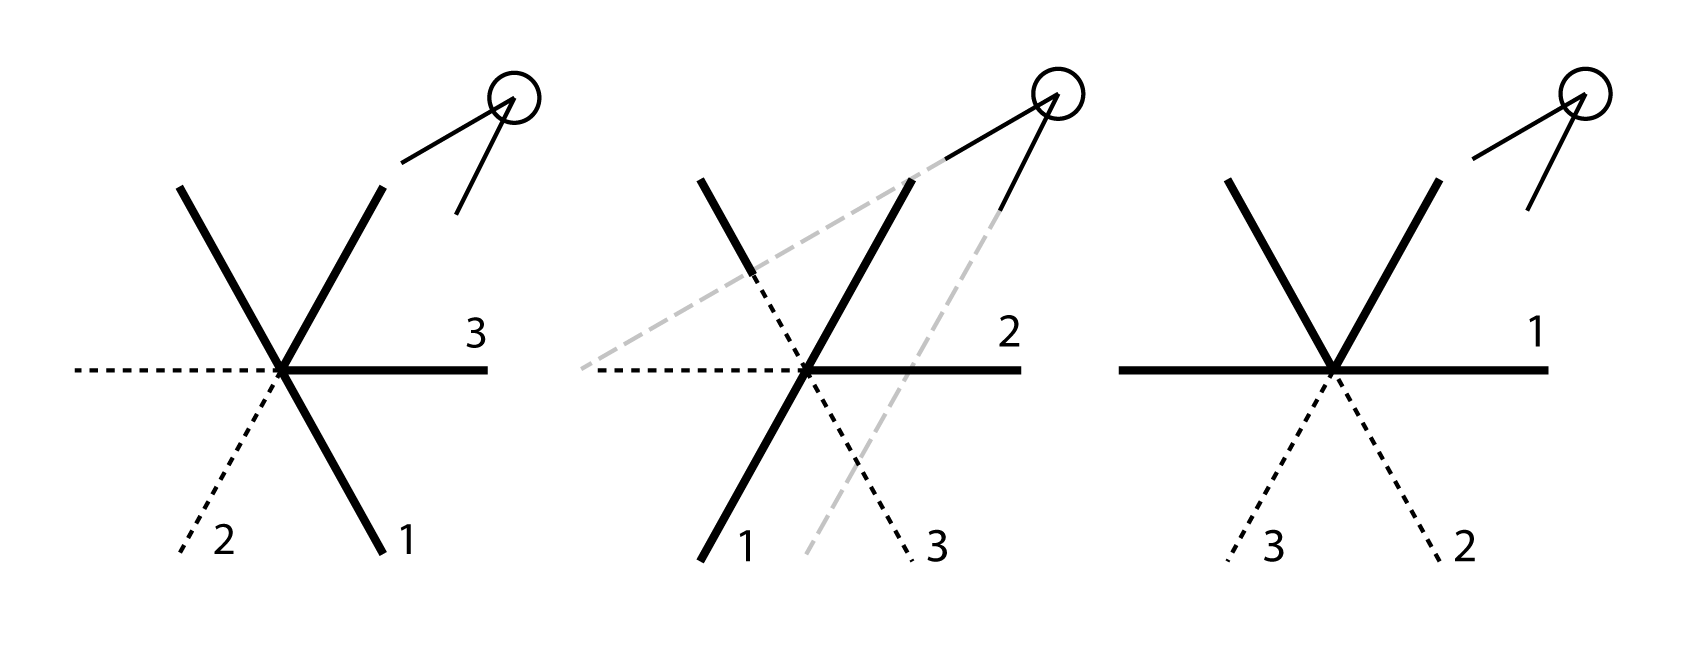
\includegraphics[width=0.6\textwidth]{./figures/LODtransparency.png}
\end{center}
\caption[Průhlednost trsu řezů]%
{Schematicky znázorněné problémy vykreslování průhledných, křížících se řezů. Tlustou plnou čarou jsou naznačeny správně vykreslené oblasti, tence čárkovaně oblasti, které nejsou vykresleny a mohou způsobit problémy.
\label{fig:lodSliceOrdering}
}
\end{figure}

Průhlednost mezi instancemi je ošetřena řazením v rámci zpracování instancí. Geometrická primitiva v rámci jedné instance je ovšem také třeba řadit. Jak je patrné z obrázku \ref{fig:lodSliceOrdering}, nelze pouhým řazením geometrických primitiv zajistit zcela korektní vykreslení. Ovšem důležité je si uvědomit skutečnost, že problémy způsobují zejména řezy skoro rovnoběžné s pohledem (dále jen \emph{rovnoběžný řez}), které jsou stejně skrývány (proto jsou vysoce průhledné). Zejména problematická je pak jejich část blíž k pozorovateli. Část dále od pozorovatele zakrývají řezy méně průhledné natočené víceméně kolmo ke směru pohledu. Stačí tedy zajistit, aby se takový rovnoběžný řez vykresloval až po ostatních.
\begin{figure}[!hbt]
\begin{center}
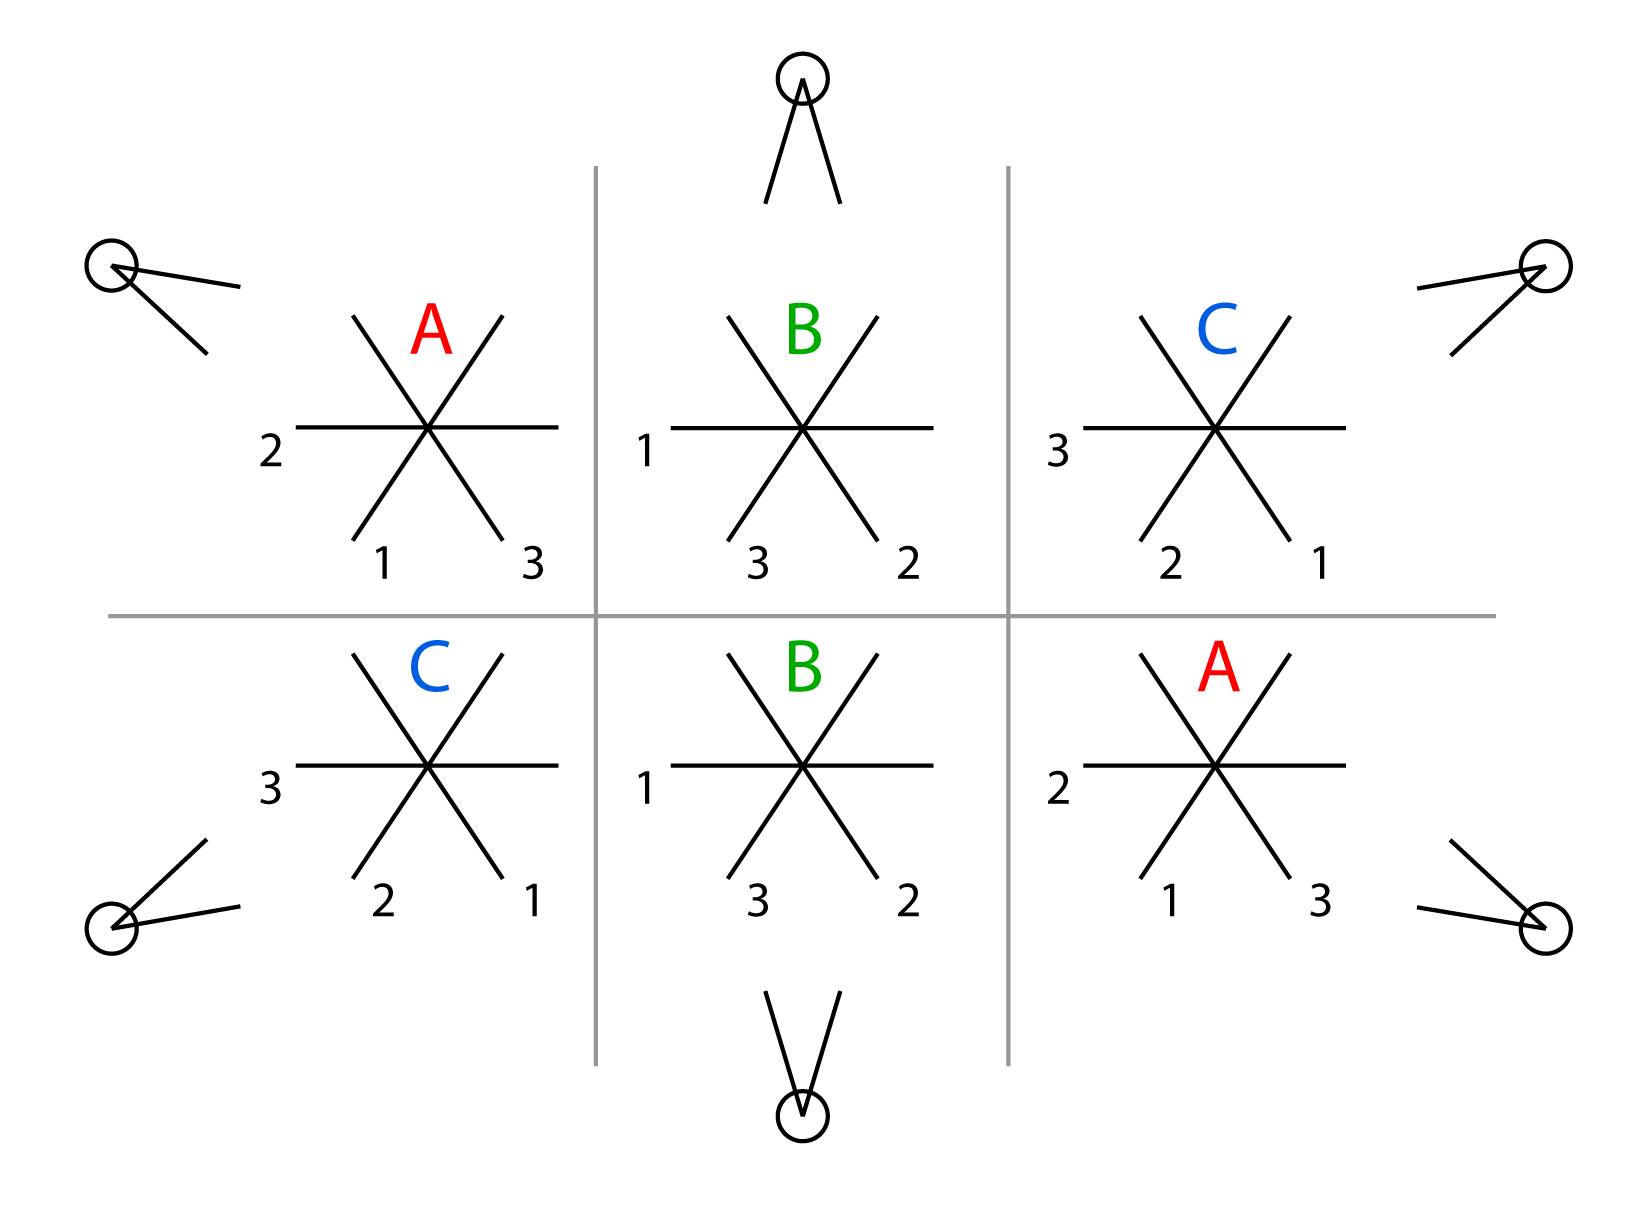
\includegraphics[width=0.6\textwidth]{./figures/LODtypes.png}
\end{center}
\caption[Variace pořadí vykreslování trsu řezů]%
{Různé případy pozice pozorovatele vůči trsu řezů. Všechny možnosti se redukují na 3 případy pořadí vykreslování řezů (A,B,C).
\label{fig:LODtypes}
}
\end{figure}
Jak je patrné z obr.~\ref{fig:LODtypes}, je třeba rozlišit, jaký případ nastává a podle toho určit pořadí vykreslení jednotlivých řezů. Fronty instancí se tedy rozpadají ještě podle tohoto kritéria (viz obr. \ref{fig:LODqueues}), neboť různé pořadí vykreslení jednotlivých řezů je zajištěno různým souborem indexů v EBO.
\begin{figure}[!hbt]
\begin{center}
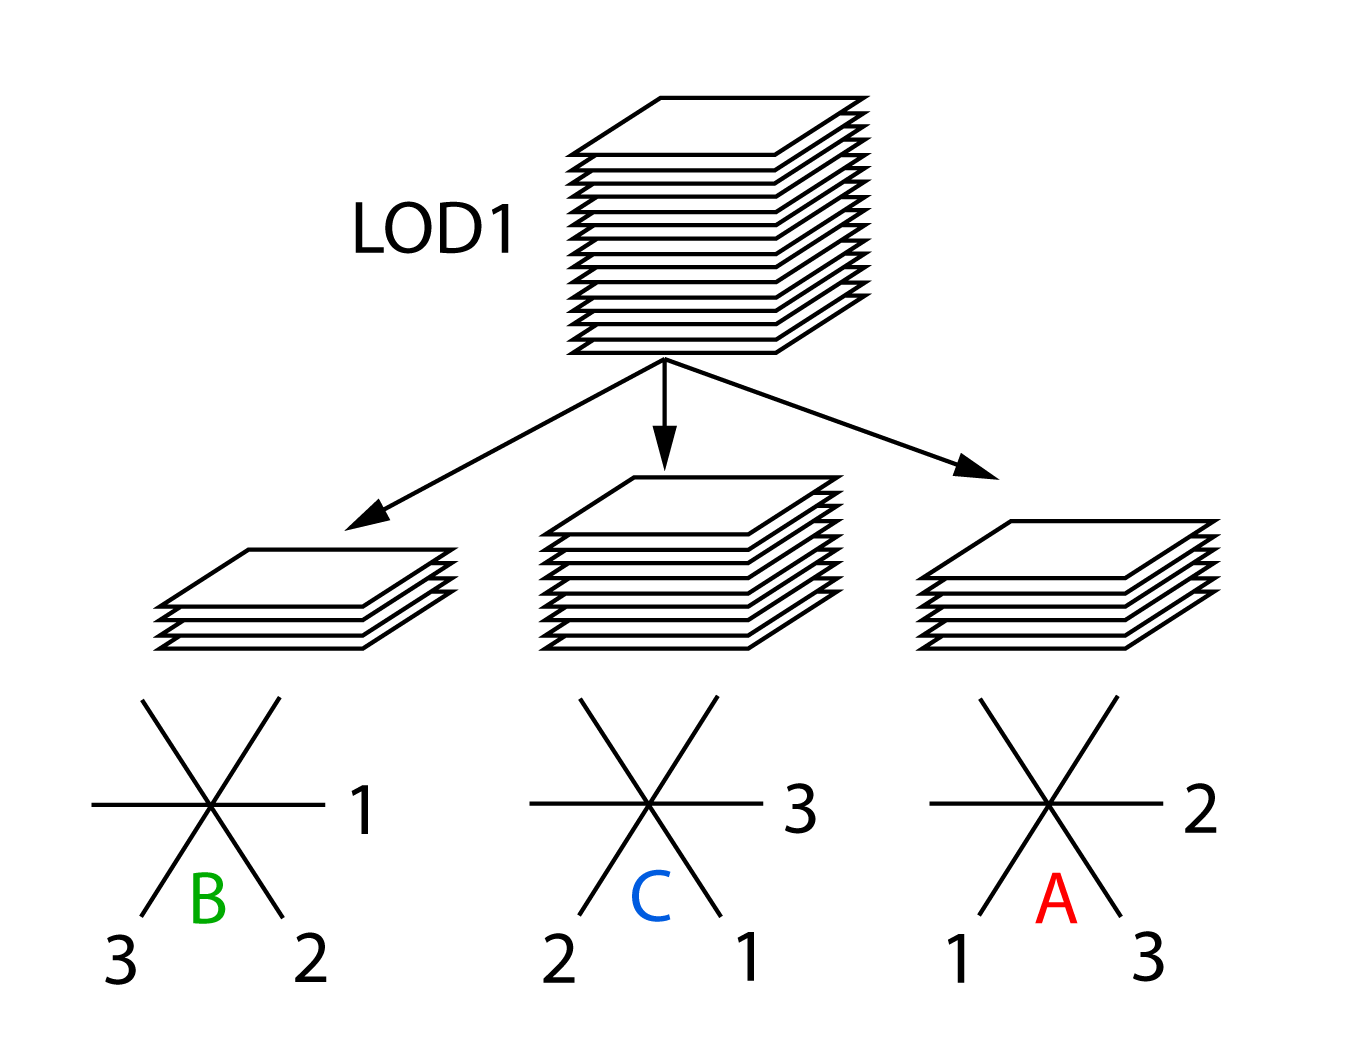
\includegraphics[width=0.4\textwidth]{./figures/renderQueuesB.png}
\end{center}
\caption[Pořadí vykreslování LOD1]%
{Rozpad fronty instancí LOD1 do několika menších front podle pořadí vykreslení (A,B,C).
\label{fig:LODqueues}
}
\end{figure}

\pagebreak
Samotné vykreslování a animace jednotlivých instancí LOD1 a LOD2 probíhá rovněž pomocí speciálního \emph{shaderu} (programu na GPU). Existuje stejný shader jak pro vykreslování instancované, tak i neinstancované geometrie. Odlišnosti chování se projevují pouze ve \emph{vertex shaderu} (prefixy \lineCode{ia} označují instanční atributy):
\begin{alltt}
\textit{// color_variance\dots uniformni parametr, barevna odchylka instance}
\textit{// time_offset\dots uniformni parametr, casova odchylka instance}
\textit{// wind_direction\dots uniformni parametr, smer vetru}
\textit{// ia_transform_matrix\dots instancni atribut, transformacni matice instance}
\textit{// ia_wind_matrix\dots instancni atribut, transformacni matice otoceni smeru vetru}

if (isInstancingActive)\{
    \textit{// kresli se v modu instancovane geometrie}
    color_variance = ia_color_variance.rgb;
    time_offset    = ia_time_offset;
  
    position = gl_ModelViewMatrix * (ia_transform_matrix * position);
    mat3 T   = gl_NormalMatrix * mat3(ia_transform_matrix);
		
    tangent    = ( T * tangent );
    normal     = ( T * normal ); 
    bitangent	 = ( T * bitangent );

    wind_direction = mat3(ia_transform_matrix) * ia_wind_matrix * wind_direction;
\} else \{
    \textit{// kresli jednotlive instance}
    position   = gl_ModelViewMatrix * position;
    tangent    = ( gl_NormalMatrix * tangent );
    normal     = ( gl_NormalMatrix * normal );		
    bitangent  = ( gl_NormalMatrix * bitangent );
\}
\end{alltt}
Jak již bylo naznačeno v sekci~\ref{sec:preprocessLOD}, jsou textury využívané ve \emph{fragment shaderu} slučeny po skupinách. Je tedy nutné v rámci fragment shaderu rozlišit, jaký řez je aktuálně kreslen a podle toho transformovat souřadnice dotazů do takových sloučených textur (mapovat původní rozsah $\left< 0-1 \right >$ do příslušné oblasti sloučené textury). Informaci o právě kresleném řezu lze předat do fragment shaderu pomocí atributů vrcholů. Stačí použít dvousložkový vektor, kde první složka definuje, která sada řezů je aktivní (z jakého směru) a druhá složka určuje vrstvu. To zajišťuje funkce \lineCode{sliceCoordsToTextureCoords}:
\begin{alltt}
\textit{// va_sliceDescription\dots vertexový atribut, popisuje právě kreslený řez }
\textit{// u_sliceCnt\dots uniformní parametr, počet řezů z jednoho směru }
\textit{// u_sliceSetCnt\dots uniformní parametr, počet sad řezů (směrů) }
vec2 {\bf sliceCoordsToTextureCoords}(in vec2 sliceCoords)\{
  return ( clamp ( sliceCoords, 0.0, 1.0 ) + va_sliceDescription) 
            / vec2( u_sliceCnt , u_sliceSetsCnt );
\}
\end{alltt}

Zatímco animace geometrického modelu probíhá ve vertex shaderu, ohyb větví v LOD1 a LOD2 musí probíhat ve fragment shaderu. Klíčová je funkce \lineCode{animateBranch}:
\begin{alltt}
\textit{// position\dots pozice fragmentu}
\textit{// time\dots cas}
\textit{// offset\dots identifikator sady rezu}
\textit{// texCol\dots prepocetni koeficient do textury}
\textit{// wood_a\dots amplituda pohybu }
\textit{// wood_f\dots frekvence pohybu }
\textit{// wind_d\dots smer vetru }
\textit{// wind_s\dots sila vetru }
\textit{// time\dots uniformní parametr, počet sad řezů (směrů) }
\textit{// time\dots uniformní parametr, počet sad řezů (směrů) }
\textit{// u_sliceSetCnt\dots uniformní parametr, počet sad řezů (směrů) }

void {\bf animateBranch}(inout vec2 position, in float branchID, in float time,
                      in float offset, in float texCol, in float wood_a,
                      in float wood_f, in vec3 wind_d, in float wind_s)\{
    float x, lengthP;
    vec2 mv, corr_s, corr_r, amp, origin, t, amp, fu, fu_deriv;
    vec3 r, s;
    vec4 b_data0, b_data1, b_data2, b_data3;
\textit{// nacteni dat o vetvi z textur }
    b_data0 = texture2D(lod_data_tex, vec2((0.5+offset)*texCol, branchID));
    b_data1 = texture2D(lod_data_tex, vec2((1.5+offset)*texCol, branchID));
    b_data2 = texture2D(lod_data_tex, vec2((2.5+offset)*texCol, branchID));
    origin = b_data0.xy;
    mv = b_data0.zw;
    r = b_data1.xyz;
    s = b_data2.xyz;
    t = cross(s,r).xy;
    lengthP = b_data1.w;
\textit{// hodnota x}		
    x = min(1.0, length(abs(position-origin))/lengthP);
\textit{// vychylka}	
    amp = vec2(dot(r, wind_d) * wind_s, dot(s, wind_d) * wind_s);
    amp += wood_a * ( texture2D( branch_noise_tex , mv * time * wood_f).rg  * 2.0 - vec2(1.0) );
\textit{// ohybova funkce}	
    float x2 = x * x;
    float fx = 0.374570*x2 + 0.129428*x2*x2;
    float dx = 0.749141*x + 0.517713*x2*x;
    fu = vec2(fx) * amp;
    fu_deriv = vec2( dx / lengthP ) * amp;
\textit{// zamezeni deleni nulou}	
    fu_deriv = max(fu_deriv, EPSILON) + min(fu_deriv, EPSILON);
\dots
\pagebreak
\textit{// korekce delky}
    vec2 us = sqrt( vec2(1.0) + fu_deriv * fu_deriv );
    vec2 ud = fu / fu_deriv * ( us - vec2(1.0) );
    corr_r = ( t + r.xy * fu_deriv.x ) / us.x * ud.x;
    corr_s = ( t + s.xy * fu_deriv.y ) / us.y * ud.y;
\textit{// ohyb - POZOR: zpetna transformace musi pusobit proti puvodni}
    position = position - ( fu.x * r.xy + fu.y * s.xy - ( corr_r + corr_s ) );
\}
\end{alltt}

Tato funkce je aplikována dvakrát, nejprve na 1. úroveň větví, poté na kmen. Tedy opačně než v případě deformace geometrického modelu. S tím souvisí problém aplikace směrové složky větru. Zatímco správně je deformován nejprve kmen a s ním i souřadné systémy napojených větví a tím pádem se průmět směru větru na větve 1. úrovně mění s deformací kmene. V LOD1 a LOD2 však je aplikována směrová složka větru na větve na neohnutém kmeni a teprve poté je ohnut kmen. Tato chyba však nezpůsobuje příliš velký problém a je skoro nepostřehnutelná.

%%%%%%
% sezoni zmeny barev + barevne variace
%
\section{Sezónní barvy a barevné variace}
Vegetace (stromy nevyjímaje) podléhá změnám během ročních období. Tato sekce popisuje, jak zajistit změnu barevnosti listů, která je daná roční dobou (sezónou), a jak zajistit, aby se mírně lišila barevnost jednak listů mezi sebou, ale i celková barevnost jednotlivých stromů mezi sebou. 

Jak již bylo naznačeno v předchozím textu, sezónní barva je definovaná texturou (viz obr.~\ref{fig:seasonMap}) a souřadnicí, ze které se příslušná barva získává. Sezónu definuje parametr \lineCode{season}. Pro zajištění barevných variací mezi jednotlivými listy je třeba přiřadit listu specifické číslo \lineCode{leafSpecificNumber}. Toto číslo je třeba distribuovat i do textur používaných pro zobrazení řezů. Využije se k tomu s výhodou 4. složka textury normál. Odchylku barevnosti celých stromů mezi sebou zajistíme podobným mechanismem. Ten je společný i pro zajištění odchylky ve fázi animace. Instanci tak přísluší \lineCode{instanceSpecificNumber}. Pomocí těchto proměnných lze zajistit odchylku od přímé sezónní barvy:
\begin{alltt}
float seasonCoord = season + 0.2*leafSpecificNumber
                                             - 0.0001*instanceSpecificNumber;
vec4  seasonColor = texture2D(seasonMap, vec2(0.5, seasonCoord);
\end{alltt}
Koeficienty váhy jednotlivých odchylek byly určeny pouze na základě výsledného vizuálního dojmu a pro různé textury sezónních barev mohou být rozdílné.

Touto metodou lze velmi jednoduše zajistit i přibývání počtu listů na jaře a naopak snižování počtu listů na podzim. Stačí, když je příslušná část textury sezónní barvy průhledná. Pokud je tedy výsledná sezónní barva průhledná, je zpracovávaný fragment zahozen:
\begin{alltt}
  if ( seasonColor.a < 0.5 )\{
     discard;
  \}
\end{alltt}

%%%%%%
%  stiny...
%
\section{Stíny}
Stíny mají velký vliv na vizuální kvalitu generovaného obrazu a jejich věrnost může použitím trsů řezů velmi utrpět. Standardní technikou generující dynamicky stíny je tzv. \emph{shadow-mapping}. Je generována stínová mapa jako záznam vzdálenosti fragmentů od zdroje světla. Následně je pro daný zobrazovaný bod porovnávána vzdálenost od světla $D_L$ se záznamem na odpovídajícím místě stínové mapy $D_S$ (viz obr.~\ref{fig:shadowMapping}).
\begin{figure}[!hbt]
\begin{center}
$\begin{array}{cc}
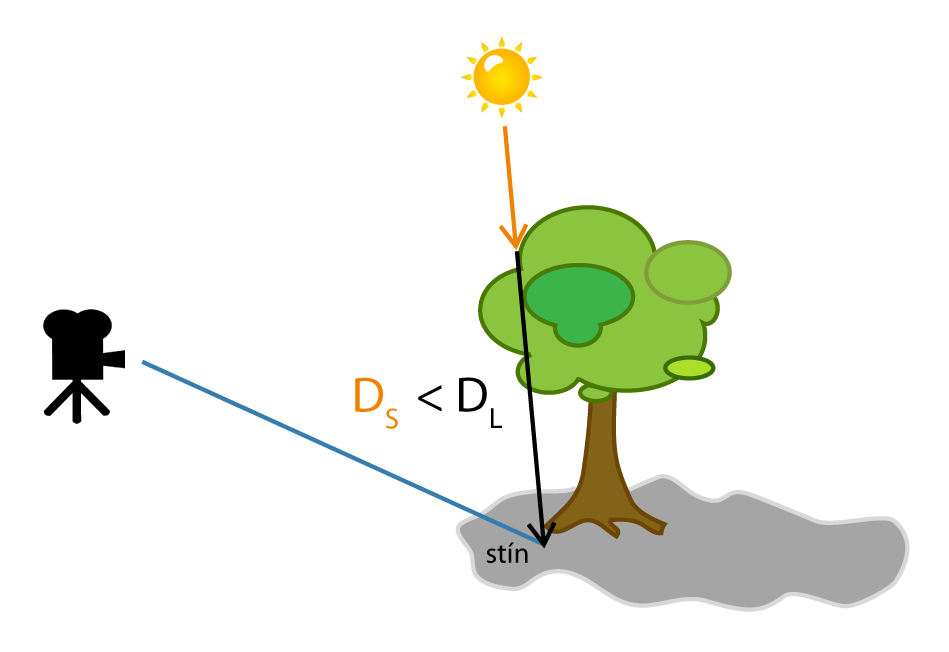
\includegraphics[width=0.45\textwidth]{./figures/shadowMapping.png}&
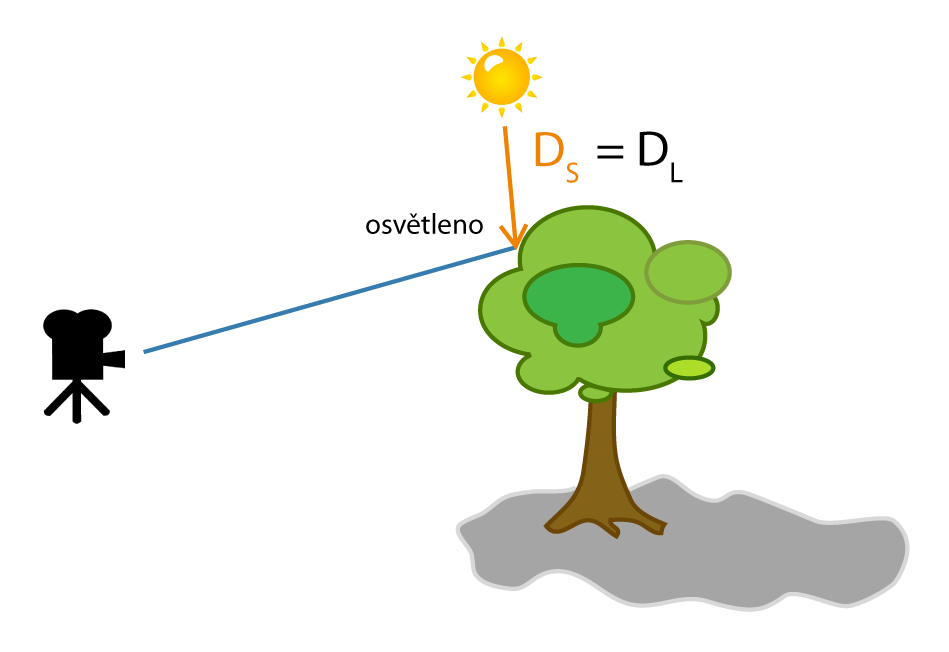
\includegraphics[width=0.45\textwidth]{./figures/shadowMapping2.png}\\
(a)&(b)
\end{array}$
\end{center}
\caption[Princip shadow mappingu]%
{Princip shadow mappingu. (a) vdálenost zobrazovaného bodu ke světlu je větší než záznam ve stínové mapě - bod leží ve stínu, (b) vzdálenosti jsou shodné - bod je osvětlen.
\label{fig:shadowMapping}
}
\end{figure}

Pokud uvažujeme pouze světla, která nesvítí na trs řezů přímo zvrchu, generuje i tato primitivní konstrukce relativně dobře vypadající stíny. Problém ovšem nastává ve stínech na stromu samotném. Na geometrickém modelu je jasně patrné, že některé části koruny stromu jsou ve stínu. S určitými kompromisy je možné dosáhnout podobného efektu i pro ploché řezy. Klíčové je zapsat do stínové mapy nikoliv přímo hloubku plochy řezu, ale posunout hloubku ještě o příslušnou hodnotu získanou z hloubkové mapy řezu. Stejný princip se uplatňuje i při vyhodnocování, kde je rovněž dobré hodnotu posunout. Hloubku lze do stínové mapy zapsat jednoduše přiřazením do proměnné \lineCode{gl\_FragDepth = hodnota}. Tato operace však může zapříčinit zpomalení celého procesu zobrazení, neboť GPU provádí sérii optimalizací, mezi kterými je i tzv. \emph{early z-test}. Provedení této optimalizační techniky, která probíhá před spuštením fragment shaderu a případně ho vůbec nespouští, je vázáno na podmínku, že hloubka fragmentu není ve fragment shaderu měněna.

%%%%
%	porovnání stínů
%
\begin{figure}[!hbt]
\begin{center}
$\begin{array}{cc}
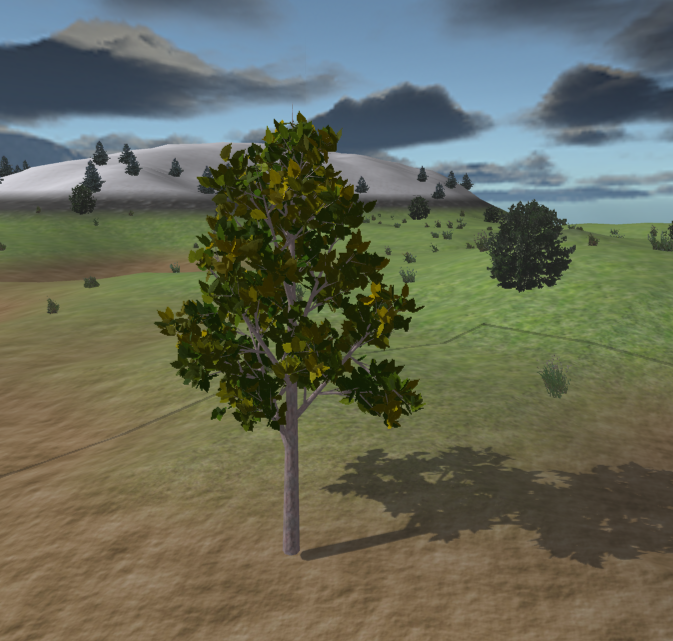
\includegraphics[width=0.45\textwidth]{./figures/shadowsLOD0.png}&
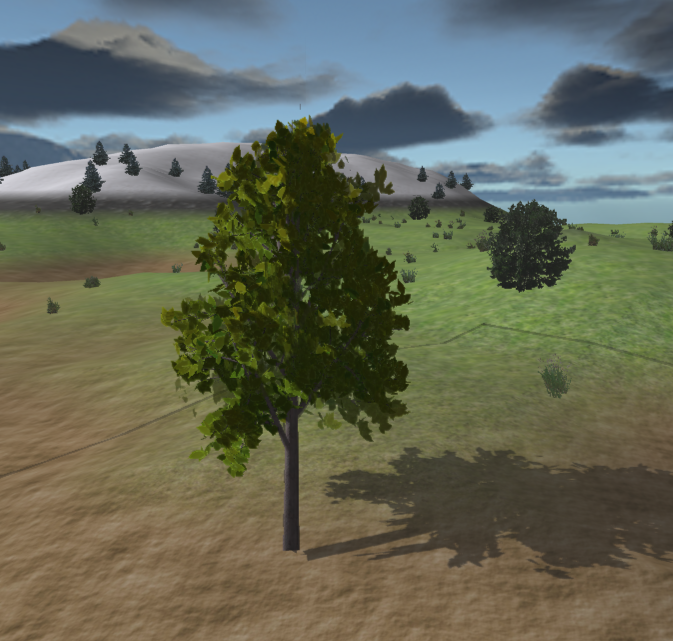
\includegraphics[width=0.45\textwidth]{./figures/shadowsLOD1.png}\\
(a)&(b)
\end{array}$
\end{center}
\caption[Stíny v LOD0 a LOD1]%
{Porovnání stínů LOD0 (a) a LOD1 (b).
\label{fig:shadowMapping}
}
\end{figure}
\pagebreak
Stíny mohou vytvářet problém i při plynulém přechodu mezi úrovněmi LOD. Jde o to, že zatímco barevný obraz se plynule prolíná pomocí průhlednosti, ve stínové hloubkové mapě žádná průhlednost nefunguje. Děje se tak skoková změna v zápisu do stínové mapy a tím je ovlivněn i barevný obraz jež je skokově jinak stínován. Tento nepříjemný efekt lze částečně potlačit využitím tónování (tzv. \emph{dithering}). Tímto způsobem lze simulovat průhlednost i bez kanálu průhlednosti. Z plochy, která má být průhledná, je odebrán náhodně určitý počet pixelů (jsou plně průhledné), podle hodnoty požadované průhlednosti. Čím má být plocha průhlednější, tím víc pixelů je takto odstaněno. Pokud je touto řídící veličinou proměnná \lineCode{transition\_control}, pak lze tónování stínové mapy docílit takto:
\begin{alltt}
\textit{// noise\dots náhodné číslo stejného rozsahu jako transition\_control}
    if ( transition_control < noise ) \{
        discard;
    \}
\end{alltt}
